\documentclass[sigconf]{acmart}

\usepackage{algorithmic}
\usepackage{algorithm}
\usepackage{hyperref}
\usepackage{listings}

\begin{document}

\title{Lab 8 Exercise - Exploring Latent Spaces}
\author{Luke McClure}
\email{29573904}

\maketitle
\pagestyle{myheadings}

\begin{figure}
    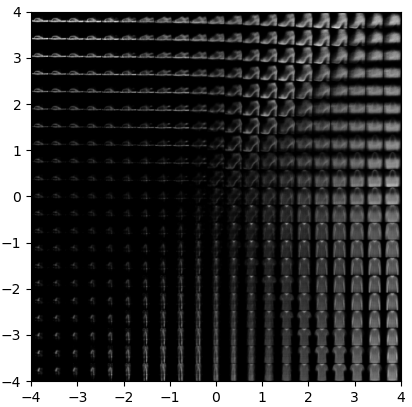
\includegraphics[width=.4\textwidth]{../VAE.png}
    \caption{VAE latent space}
    \label{fig:VAE}
\end{figure}
\begin{figure}
    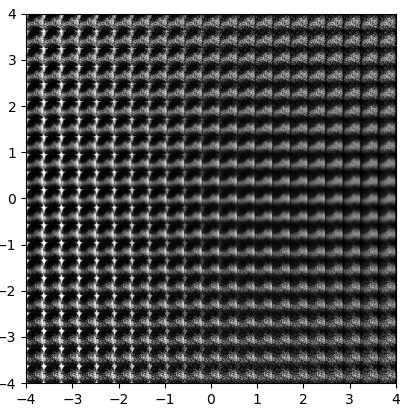
\includegraphics[width=.4\textwidth]{../AE.png}
    \caption{Autoencoder latent space}
    \label{fig:AE}
\end{figure}
\section{Compare the latent spaces of the VAE and autoencoder}
There are a number of differences between the latent space of the VAE displayed in \autoref{fig:VAE} and the latent space of the autoencoder in \autoref{fig:AE}.
\begin{itemize}
    \item Feature discernability\\
        Within the latent space of the VAE there are several distinctive classes that can be seen, with a collection of different types of shoes across the top of the image and various styles of top across the right hand side.
        This is in stark contrast to the latent space of the AE, where the only class that can be clearly made out are the shoes close to centre right in \autoref{fig:AE}.\\
    \item Feature brightness\\
        Opposed to discernability, the latent space of the AE appears to be a lot brighter than that of the VAE. 
        This aids in the discernability of features for the VAE latent space, where it is a lot easier to see the feature against the dark background with varying shades of greys compared to the stark white of the AE latent space.\\
    \item Class boundaries\\
        Within the VAE latent space there is not only a notion of class boundaries, but the transition between them are smooth and sensible. 
        Mentioned previously was the band of shoes across the top of \autoref{fig:VAE}, digging deeper into this band it is clear to see how flip flops on the left side start to form into high heels and then boots going from left to right.
        This pattern follows down the right side where several forms of top meld together.

        This is in contrast to the AE latent space, where there is little notion of different classes nevermind class boundaries. The only distinctive class within this part of the latent space is the shoes mentioned previously, but there seems to be no class bordering it within the scope of this sample.
\end{itemize}

The sampled VAE encoder latent space distribution is centred around a mean of 0,0, with the gaussian sampling acting to tighten the distribution around this origin point. This has the effect of bringing the transition of classes into much clearer view, improving both feature discernability as well as the class boundaries on display.
It is also able to tie like features close together, such as the heel of boots, flat bottom of shoes and general shape of tops into distinct areas of the latent space.

The AE latent space does not seem to have these same properties, with only the shoes appearing in a small part of this sample while the rest of the latent space seems to drift progressively away from that general shape. Without the gaussian centering and tightening of the distribution I imagine with a much larger sample size than +/-4 in either dimension then the other classes may be captured.

\end{document}
\endinput